\documentclass{standalone}
\usepackage{tikz}
\usetikzlibrary{patterns, positioning}

\begin{document}
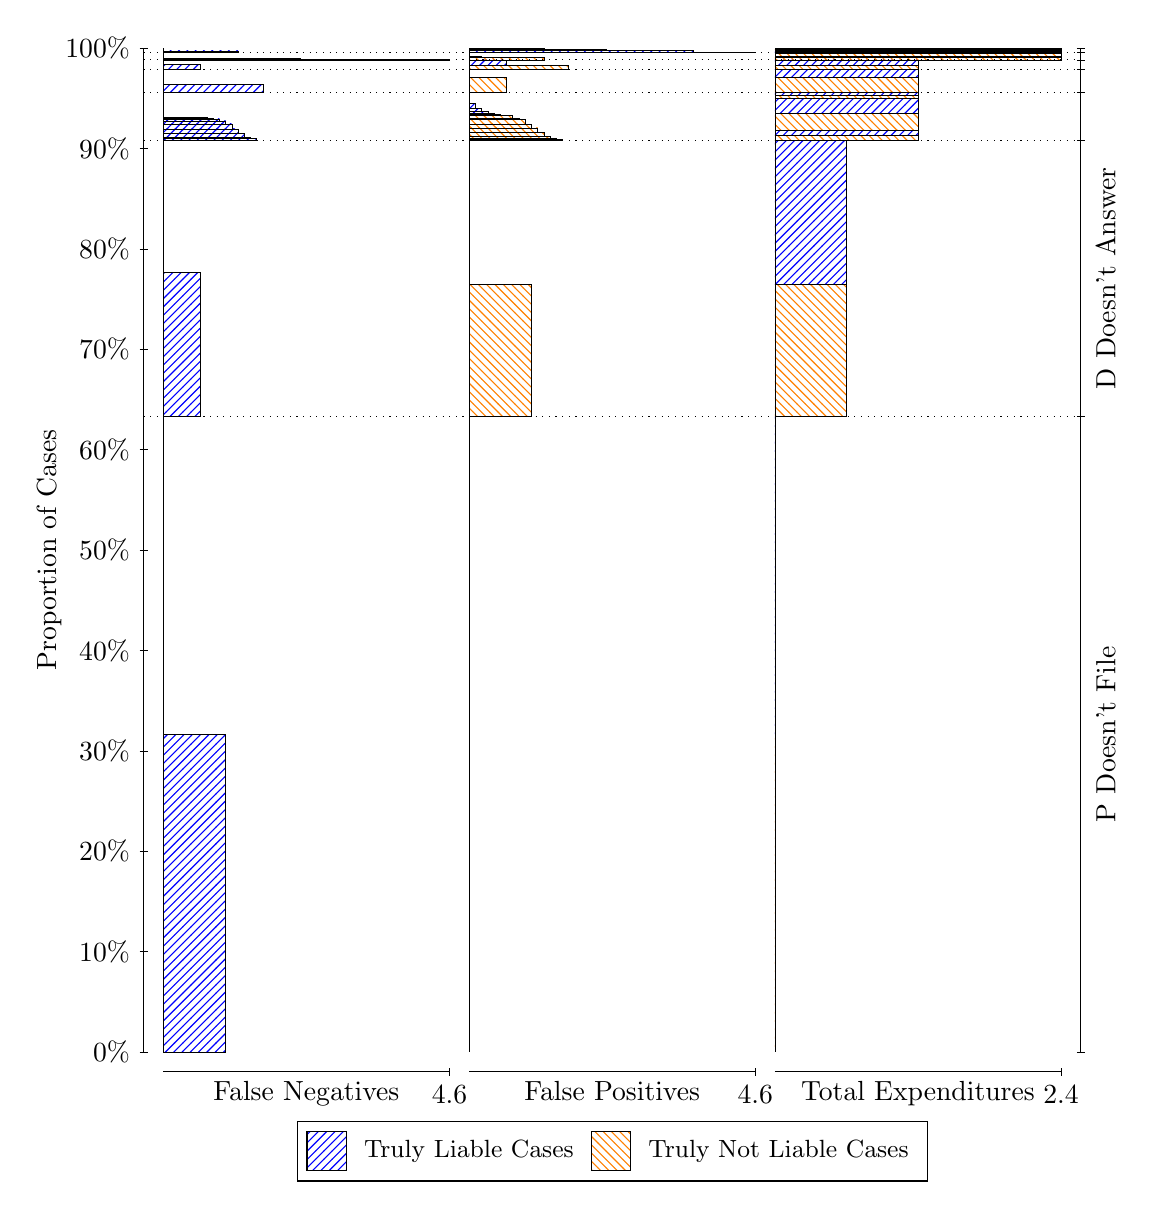
\begin{tikzpicture}
\draw[black, very thin] (1.5,1.75) -- (1.5,14.5);
\node[rotate=90, anchor=center] at (0.3, 8.125) {Proportion of Cases};
\draw[black, very thin] (1.45,1.75) -- (1.55,1.75);
\node[anchor=east] at (1.45, 1.75) {0\%};
\draw[black, very thin] (1.45,3.025) -- (1.55,3.025);
\node[anchor=east] at (1.45, 3.025) {10\%};
\draw[black, very thin] (1.45,4.3) -- (1.55,4.3);
\node[anchor=east] at (1.45, 4.3) {20\%};
\draw[black, very thin] (1.45,5.575) -- (1.55,5.575);
\node[anchor=east] at (1.45, 5.575) {30\%};
\draw[black, very thin] (1.45,6.85) -- (1.55,6.85);
\node[anchor=east] at (1.45, 6.85) {40\%};
\draw[black, very thin] (1.45,8.125) -- (1.55,8.125);
\node[anchor=east] at (1.45, 8.125) {50\%};
\draw[black, very thin] (1.45,9.4) -- (1.55,9.4);
\node[anchor=east] at (1.45, 9.4) {60\%};
\draw[black, very thin] (1.45,10.675) -- (1.55,10.675);
\node[anchor=east] at (1.45, 10.675) {70\%};
\draw[black, very thin] (1.45,11.95) -- (1.55,11.95);
\node[anchor=east] at (1.45, 11.95) {80\%};
\draw[black, very thin] (1.45,13.225) -- (1.55,13.225);
\node[anchor=east] at (1.45, 13.225) {90\%};
\draw[black, very thin] (1.45,14.5) -- (1.55,14.5);
\node[anchor=east] at (1.45, 14.5) {100\%};

\draw[black, very thin] (13.4,1.75) -- (13.4,14.5);
\draw[black, very thin] (13.35,1.75) -- (13.45,1.75);
\node[anchor=west] at (13.35, 1.75) {};
\draw[black, very thin] (13.35,9.8202) -- (13.45,9.8202);
\node[anchor=west] at (13.35, 9.8202) {};
\draw[black, very thin] (13.35,13.331) -- (13.45,13.331);
\node[anchor=west] at (13.35, 13.331) {};
\draw[black, very thin] (13.35,13.935) -- (13.45,13.935);
\node[anchor=west] at (13.35, 13.935) {};
\draw[black, very thin] (13.35,14.23) -- (13.45,14.23);
\node[anchor=west] at (13.35, 14.23) {};
\draw[black, very thin] (13.35,14.349) -- (13.45,14.349);
\node[anchor=west] at (13.35, 14.349) {};
\draw[black, very thin] (13.35,14.444) -- (13.45,14.444);
\node[anchor=west] at (13.35, 14.444) {};
\draw[black, very thin] (13.35,14.5) -- (13.45,14.5);
\node[anchor=west] at (13.35, 14.5) {};

\draw[black, very thin, pattern color=blue, pattern=north east lines] (1.75,1.75) rectangle (2.5399,5.7851);
\draw[black, very thin, pattern color=orange, pattern=north west lines] (1.75,5.7851) rectangle (1.75,9.8202);
\draw[black, very thin, pattern color=blue, pattern=north east lines] (1.75,9.8202) rectangle (2.2239,11.649);
\draw[black, very thin, pattern color=orange, pattern=north west lines] (1.75,11.649) rectangle (1.75,13.331);
\draw[black, very thin, pattern color=blue, pattern=north east lines] (1.75,13.331) rectangle (2.9348,13.351);
\draw[black, very thin, pattern color=blue, pattern=north east lines] (1.75,13.351) rectangle (2.8558,13.366);
\draw[black, very thin, pattern color=blue, pattern=north east lines] (1.75,13.366) rectangle (2.7768,13.419);
\draw[black, very thin, pattern color=blue, pattern=north east lines] (1.75,13.419) rectangle (2.6978,13.473);
\draw[black, very thin, pattern color=blue, pattern=north east lines] (1.75,13.473) rectangle (2.6188,13.537);
\draw[black, very thin, pattern color=blue, pattern=north east lines] (1.75,13.537) rectangle (2.5399,13.574);
\draw[black, very thin, pattern color=blue, pattern=north east lines] (1.75,13.574) rectangle (2.4609,13.599);
\draw[black, very thin, pattern color=blue, pattern=north east lines] (1.75,13.599) rectangle (2.3819,13.609);
\draw[black, very thin, pattern color=blue, pattern=north east lines] (1.75,13.609) rectangle (2.3029,13.619);
\draw[black, very thin, pattern color=orange, pattern=north west lines] (1.75,13.619) rectangle (1.75,13.935);
\draw[black, very thin, pattern color=blue, pattern=north east lines] (1.75,13.935) rectangle (3.0138,14.035);
\draw[black, very thin, pattern color=orange, pattern=north west lines] (1.75,14.035) rectangle (1.75,14.23);
\draw[black, very thin, pattern color=blue, pattern=north east lines] (1.75,14.23) rectangle (2.2239,14.297);
\draw[black, very thin, pattern color=orange, pattern=north west lines] (1.75,14.297) rectangle (1.75,14.349);
\draw[black, very thin, pattern color=blue, pattern=north east lines] (1.75,14.349) rectangle (5.3833,14.353);
\draw[black, very thin, pattern color=blue, pattern=north east lines] (1.75,14.353) rectangle (3.4877,14.364);
\draw[black, very thin, pattern color=orange, pattern=north west lines] (1.75,14.364) rectangle (1.75,14.444);
\draw[black, very thin, pattern color=blue, pattern=north east lines] (1.75,14.444) rectangle (2.6978,14.463);
\draw[black, very thin, pattern color=orange, pattern=north west lines] (1.75,14.463) rectangle (1.75,14.478);
\draw[black, very thin, pattern color=blue, pattern=north east lines] (1.75,14.478) rectangle (1.75,14.5);
\draw[black, very thin, pattern color=orange, pattern=north west lines] (5.6333,1.75) rectangle (5.6333,5.7852);
\draw[black, very thin, pattern color=blue, pattern=north east lines] (5.6333,5.7852) rectangle (5.6333,9.8202);
\draw[black, very thin, pattern color=orange, pattern=north west lines] (5.6333,9.8202) rectangle (6.4232,11.503);
\draw[black, very thin, pattern color=blue, pattern=north east lines] (5.6333,11.503) rectangle (5.6333,13.331);
\draw[black, very thin, pattern color=orange, pattern=north west lines] (5.6333,13.331) rectangle (6.8181,13.342);
\draw[black, very thin, pattern color=orange, pattern=north west lines] (5.6333,13.342) rectangle (6.7391,13.354);
\draw[black, very thin, pattern color=orange, pattern=north west lines] (5.6333,13.354) rectangle (6.6601,13.38);
\draw[black, very thin, pattern color=orange, pattern=north west lines] (5.6333,13.38) rectangle (6.5812,13.426);
\draw[black, very thin, pattern color=orange, pattern=north west lines] (5.6333,13.426) rectangle (6.5022,13.487);
\draw[black, very thin, pattern color=orange, pattern=north west lines] (5.6333,13.487) rectangle (6.4232,13.538);
\draw[black, very thin, pattern color=orange, pattern=north west lines] (5.6333,13.538) rectangle (6.3442,13.593);
\draw[black, very thin, pattern color=orange, pattern=north west lines] (5.6333,13.593) rectangle (6.2652,13.607);
\draw[black, very thin, pattern color=orange, pattern=north west lines] (5.6333,13.607) rectangle (6.1862,13.647);
\draw[black, very thin, pattern color=blue, pattern=north east lines] (5.6333,13.647) rectangle (6.0283,13.657);
\draw[black, very thin, pattern color=blue, pattern=north east lines] (5.6333,13.657) rectangle (5.9493,13.667);
\draw[black, very thin, pattern color=blue, pattern=north east lines] (5.6333,13.667) rectangle (5.8703,13.692);
\draw[black, very thin, pattern color=blue, pattern=north east lines] (5.6333,13.692) rectangle (5.7913,13.729);
\draw[black, very thin, pattern color=blue, pattern=north east lines] (5.6333,13.729) rectangle (5.7123,13.793);
\draw[black, very thin, pattern color=blue, pattern=north east lines] (5.6333,13.793) rectangle (5.6333,13.935);
\draw[black, very thin, pattern color=orange, pattern=north west lines] (5.6333,13.935) rectangle (6.1072,14.13);
\draw[black, very thin, pattern color=blue, pattern=north east lines] (5.6333,14.13) rectangle (5.6333,14.23);
\draw[black, very thin, pattern color=orange, pattern=north west lines] (5.6333,14.23) rectangle (6.8971,14.282);
\draw[black, very thin, pattern color=blue, pattern=north east lines] (5.6333,14.282) rectangle (6.1072,14.349);
\draw[black, very thin, pattern color=orange, pattern=north west lines] (5.6333,14.349) rectangle (6.5812,14.382);
\draw[black, very thin, pattern color=blue, pattern=north east lines] (5.6333,14.382) rectangle (5.7913,14.392);
\draw[black, very thin, pattern color=orange, pattern=north west lines] (5.6333,14.392) rectangle (5.6333,14.439);
\draw[black, very thin, pattern color=blue, pattern=north east lines] (5.6333,14.439) rectangle (5.6333,14.444);
\draw[black, very thin, pattern color=orange, pattern=north west lines] (5.6333,14.444) rectangle (9.2667,14.447);
\draw[black, very thin, pattern color=blue, pattern=north east lines] (5.6333,14.447) rectangle (8.4768,14.469);
\draw[black, very thin, pattern color=orange, pattern=north west lines] (5.6333,14.469) rectangle (7.371,14.481);
\draw[black, very thin, pattern color=blue, pattern=north east lines] (5.6333,14.481) rectangle (6.5812,14.5);
\draw[black, very thin, pattern color=orange, pattern=north west lines] (9.5167,1.75) rectangle (9.5167,5.7852);
\draw[black, very thin, pattern color=blue, pattern=north east lines] (9.5167,5.7852) rectangle (9.5167,9.8202);
\draw[black, very thin, pattern color=orange, pattern=north west lines] (9.5167,9.8202) rectangle (10.425,11.503);
\draw[black, very thin, pattern color=blue, pattern=north east lines] (9.5167,11.503) rectangle (10.425,13.331);
\draw[black, very thin, pattern color=orange, pattern=north west lines] (9.5167,13.331) rectangle (11.333,13.393);
\draw[black, very thin, pattern color=blue, pattern=north east lines] (9.5167,13.393) rectangle (11.333,13.456);
\draw[black, very thin, pattern color=orange, pattern=north west lines] (9.5167,13.456) rectangle (11.333,13.672);
\draw[black, very thin, pattern color=blue, pattern=north east lines] (9.5167,13.672) rectangle (11.333,13.862);
\draw[black, very thin, pattern color=orange, pattern=north west lines] (9.5167,13.862) rectangle (11.333,13.9);
\draw[black, very thin, pattern color=blue, pattern=north east lines] (9.5167,13.9) rectangle (11.333,13.935);
\draw[black, very thin, pattern color=orange, pattern=north west lines] (9.5167,13.935) rectangle (11.333,14.13);
\draw[black, very thin, pattern color=blue, pattern=north east lines] (9.5167,14.13) rectangle (11.333,14.23);
\draw[black, very thin, pattern color=orange, pattern=north west lines] (9.5167,14.23) rectangle (11.333,14.282);
\draw[black, very thin, pattern color=blue, pattern=north east lines] (9.5167,14.282) rectangle (11.333,14.349);
\draw[black, very thin, pattern color=orange, pattern=north west lines] (9.5167,14.349) rectangle (13.15,14.382);
\draw[black, very thin, pattern color=blue, pattern=north east lines] (9.5167,14.382) rectangle (13.15,14.392);
\draw[black, very thin, pattern color=orange, pattern=north west lines] (9.5167,14.392) rectangle (13.15,14.439);
\draw[black, very thin, pattern color=blue, pattern=north east lines] (9.5167,14.439) rectangle (13.15,14.444);
\draw[black, very thin, pattern color=orange, pattern=north west lines] (9.5167,14.444) rectangle (13.15,14.456);
\draw[black, very thin, pattern color=blue, pattern=north east lines] (9.5167,14.456) rectangle (13.15,14.475);
\draw[black, very thin, pattern color=orange, pattern=north west lines] (9.5167,14.475) rectangle (13.15,14.478);
\draw[black, very thin, pattern color=blue, pattern=north east lines] (9.5167,14.478) rectangle (13.15,14.5);
\draw[black, dotted] (1.5,9.8202) -- (13.4,9.8202);
\draw[black, dotted] (1.5,13.331) -- (13.4,13.331);
\draw[black, dotted] (1.5,13.935) -- (13.4,13.935);
\draw[black, dotted] (1.5,14.23) -- (13.4,14.23);
\draw[black, dotted] (1.5,14.349) -- (13.4,14.349);
\draw[black, dotted] (1.5,14.444) -- (13.4,14.444);
\draw[black, very thin] (1.75,1.5) -- (5.3833,1.5);
\node[anchor=north] at (3.5667, 1.5) {False Negatives};
\draw[black, very thin] (5.3833,1.45) -- (5.3833,1.55);
\node[anchor=north] at (5.3833, 1.45) {4.6};

\draw[black, very thin] (5.6333,1.5) -- (9.2667,1.5);
\node[anchor=north] at (7.45, 1.5) {False Positives};
\draw[black, very thin] (9.2667,1.45) -- (9.2667,1.55);
\node[anchor=north] at (9.2667, 1.45) {4.6};

\draw[black, very thin] (9.5167,1.5) -- (13.15,1.5);
\node[anchor=north] at (11.333, 1.5) {Total Expenditures};
\draw[black, very thin] (13.15,1.45) -- (13.15,1.55);
\node[anchor=north] at (13.15, 1.45) {2.4};

\node[black, centered, rotate=90] at (13.72, 5.7851) {P Doesn't File};
\node[black, centered, rotate=90] at (13.72, 11.576) {D Doesn't Answer};






\draw (7.449999999999999,1.5) node[draw=none] (baseCoordinate) {};
\begin{scope}[align=center]
        \matrix[scale=0.5, draw=black, below=0.5cm of baseCoordinate, nodes={draw}, column sep=0.1cm]{
            \node[rectangle, draw, minimum width=0.5cm, minimum height=0.5cm, pattern=north east lines, pattern color=blue] {}; &
            \node[draw=none, font=\small] (B) {Truly Liable Cases}; &
            \node[rectangle, draw, minimum width=0.5cm, minimum height=0.5cm, pattern=north west lines, pattern color=orange] {}; &
            \node[draw=none, font=\small] (B) {Truly Not Liable Cases}; \\
            };
\end{scope}

\end{tikzpicture}
\end{document}